\documentclass[14pt, a4paper]{extarticle}
\usepackage{GOST}
\usepackage{array}
\usepackage{verbatim}
\usepackage[detect-all]{siunitx}
\usepackage{amsmath}
\usepackage{amssymb}
\usepackage[utf8]{inputenc}
\usepackage{hyperref}
\usepackage{tempora}

\makeatletter
\renewcommand\@biblabel[1]{#1.}
\makeatother

\usepackage{listings}
\lstset{ 
	language=python,
	basicstyle=\small\sffamily, 
	numbers=left, 
	numberstyle=\tiny,
	stepnumber=1,
	numbersep=5pt,
	showspaces=false,            
	showstringspaces=false,      
	showtabs=false,             
	frame=single,            % рисовать рамку вокруг кода
	tabsize=4,      
	commentstyle=\color{green},
	keywordstyle=\color{blue}\textbf,
	numberstyle=\scriptsize\color{gray}, % the style that is used for the line-numbers
	rulecolor=\color{black},
	captionpos=t,
	breaklines=true,         % автоматически переносить строки 
	breakatwhitespace=false, % переносить строки по пробелу
	escapeinside={\#*}{*)} 
}


\usepackage{pgfplots}
\usepackage{filecontents}
\usetikzlibrary{datavisualization}
\usetikzlibrary{datavisualization.formats.functions}

\begin{document}
	
	\begin{table}[ht]
		\centering
		\begin{tabular}{|c|p{400pt}|} 
			\hline
			\begin{tabular}[c]{@{}c@{}} 
\includegraphics[scale=1]{source/baum.jpg} \\\end{tabular} &
			\footnotesize\begin{tabular}[c]{@{}c@{}}\textbf{Министерство~науки~и~высшего~образования~Российской~Федерации}\\\textbf{Федеральное~государственное~бюджетное~образовательное~учреждение}\\\textbf{~высшего~образования}\\\textbf{«Московский~государственный~технический~университет}\\\textbf{имени~Н.Э.~Баумана}\\\textbf{(национальный~исследовательский~университет)»}\\\textbf{(МГТУ~им.~Н.Э.~Баумана)}\\\end{tabular}  \\
			\hline
		\end{tabular}
	\end{table}
	\noindent\rule{\textwidth}{4pt}
	\noindent\rule[14pt]{\textwidth}{1pt}
	\hfill 
	\noindent
	\makebox{ФАКУЛЬТЕТ~}%
	\makebox[\textwidth][l]{\underline{~«Информатика и системы управления»~~~~~~~~~~~~~~~~~~~~~~~~~~~~~~~~~}}%
	\\
	\noindent
	\makebox{КАФЕДРА~}%
	\makebox[\textwidth][l]{\underline{~«Программное обеспечение ЭВМ и информационные технологии»~}}%
	\\
	
	\begin{center}
		\vspace{1.5cm}
		{\bf\huge Отчёт\par}
		{\bf\Large по лабораторной работе № 7\par}
		\vspace{0.7cm}
	\end{center}
	
	
	\noindent
	\makebox{\large{\bf Название:}~~~}
	\makebox[\textwidth][l]{\large\underline{~Поиск по словарю~}}\\
	
	\noindent
	\makebox{\large{\bf Дисциплина:}~~~}
	\makebox[\textwidth][l]{\large\underline{~Анализ алгоритмов~~~~~~~~~~~~~~~~~~~~~~~~~~}}\\
	
	\vspace{1.5cm}
	\noindent
	\begin{tabular}{l c c c c c}
		Студент      & ~ИУ7-55Б~               & \hspace{2.5cm} & \hspace{2cm}                 & &  Д.В. Сусликов \\\cline{2-2}\cline{4-4} \cline{6-6} 
		\hspace{3cm} & {\footnotesize(Группа)} &                & {\footnotesize(Подпись, дата)} & & {\footnotesize(И.О. Фамилия)}
	\end{tabular}
	
	\noindent
	\begin{tabular}{l c c c c}
		Преподаватель & \hspace{5cm}   & \hspace{2cm}                 & & ~~~~~~Л.Л. Волкова~~~~~~\\\cline{3-3} \cline{5-5} 
		\hspace{3cm}  &                & {\footnotesize(Подпись, дата)} & & {\footnotesize(И.О. Фамилия)}
	\end{tabular}
	
	\vspace{0.6cm}
	\begin{center}	
		\vfill
		\large \textit {Москва, 2020}
	\end{center}
	
	\thispagestyle {empty}
	\pagebreak
	
	% СОДЕРЖАНИЕ 
	\clearpage
	\tableofcontents
	
	% ВВЕДЕНИЕ
	\clearpage
	\section*{Введение}
	\addcontentsline{toc}{section}{Введение}
	Цель работы: изучение алгоритмов поиска слов в словаре\par
	В ходе лабораторной работы требуется:
	\begin{enumerate}
		\item[1)] описать алгоритм полного перебора;
		\item[2)] описать алгоритм двоичного поиска;
		\item[3)] описать алгоритм поиска слов по сегментам;
		\item[4)] реализовать 3 алгоритма поиска по словарю;
		\item[5)] провести замеры времени работы алгоритмов.
	\end{enumerate}\par
	
	% АНАЛИТИЧЕСКИЙ РАЗДЕЛ
	\clearpage
	\section{Аналитический раздел}
	В данном разделе представлено описание трех выбранных алгоритмов.
	
	\subsection{Словарь}
	Словари играют большую роль в современной культуре, в них отражаются знания, накопленные обществом на протяжении веков. Они служат целям описания и нормализации языка, содействуют повышению правильности и выразительности речи его носителей.
	
	Словарь –  справочная книга, содержащая собрание слов (или морфем, словосочетаний, идиом и т. д.), расположенных по определенному принципу, и дающая сведения об их значениях, употреблении, происхождении, переводе на др. язык и т. п. (лингвистические словари) или информацию о понятиях и предметах, ими обозначаемых, о деятелях в каких-либо областях науки, культуры и др\hyperref[Litre]{[6]}.
	
	
	\subsection{Алгоритм полного перебора}
	Алгоритм полного перебора — это алгоритм разрешения математических задач, который можно отнести к классу способов нахождения решения рассмотрением всех возможных вариантов.\par
	Под полным перебором понимается методика разрешения задач математики путем рассмотрения всех возможных вариантов. Уровень сложности при полном переборе напрямую связан с количеством допустимых решений задачи. В случае, когда область решений огромна, время полного перебора может исчисляться десятками и даже сотнями лет, и при этом итоговый результат возможно ещё не будет найден\hyperref[Litre]{[4]}.

	%https://spravochnick.ru/informatika/algoritmizaciya/algoritm_polnogo_perebora/ .
	
	\subsection{Алгоритм бинарного поиска}
	Бинарный поиск производится в упорядоченном массиве.\par	
	При бинарном поиске искомый ключ сравнивается с ключом среднего элемента в массиве. Если они равны, то поиск успешен. В противном случае поиск осуществляется аналогично в левой или правой частях массива.\par	
	Алгоритм может быть определен в рекурсивной и нерекурсивной формах.\par
	Бинарный поиск также называют поиском методом деления отрезка пополам или дихотомии.\par
	Двоичный поиск заключается в том, что на каждом шаге множество объектов делится на две части и в работе остаётся та часть множества, где находится искомый объект. Или же, в зависимости от постановки задачи, мы можем остановить процесс, когда мы получим первый или же последний индекс вхождения элемента. Последнее условие — это левосторонний/правосторонний двоичный поиск\hyperref[Litre]{[5]}.
	
	\subsection{Алгоритм поиска по сегментам}
	Суть заключается в том, что требуется разбить словарь по сегментам. Каждый сегмент подразумевает под собой первую букву слов, что в нём находятся.\par
	Поиск слова осуществляется сперва по сегменту, а затем по его содержимому.
	
	\subsection*{Вывод}
	\addcontentsline{toc}{subsection}{Вывод}
	В данном разделе были рассмотрены алгоритмы для поиска слова в словаре.
	
	\clearpage
	\section{Конструкторский раздел}
	В данном разделе показаны схемы разработанных алгоритмов.
	
	\subsection{Схемы алгоритмов}
	На Рисунке 1 представлена схема алгоритма полного перебора.
	\begin{figure}[h!]
		\centering{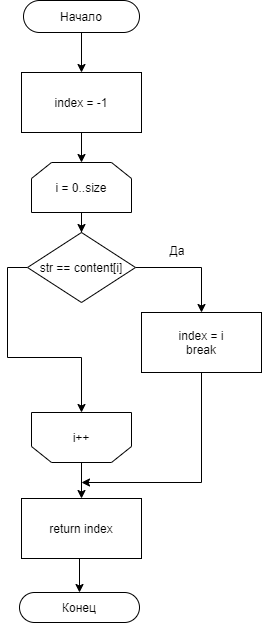
\includegraphics[scale=0.8]{source/brute.png}}
		\caption{Схема алгоритма полного перебора}
	\end{figure}
	\clearpage
	
	На Рисунке 2 показана схема алгоритма бинарного поиска.
	\begin{figure}[h!]
		\centering{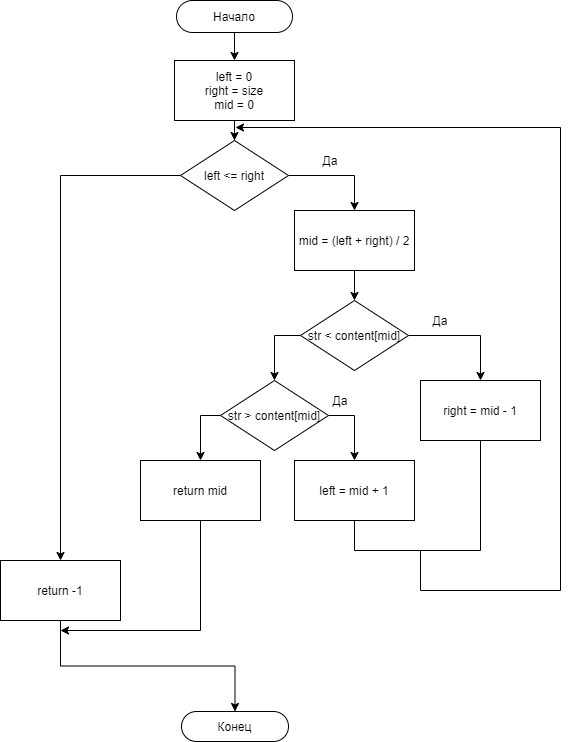
\includegraphics[scale=0.8]{source/binary.png}}
		\caption{Схема алгоритма бинарного поиска}
	\end{figure}
	\clearpage
	
	На Рисунке 3 показана схема алгоритма поиска по сегментам.
	\begin{figure}[h!]
		\centering{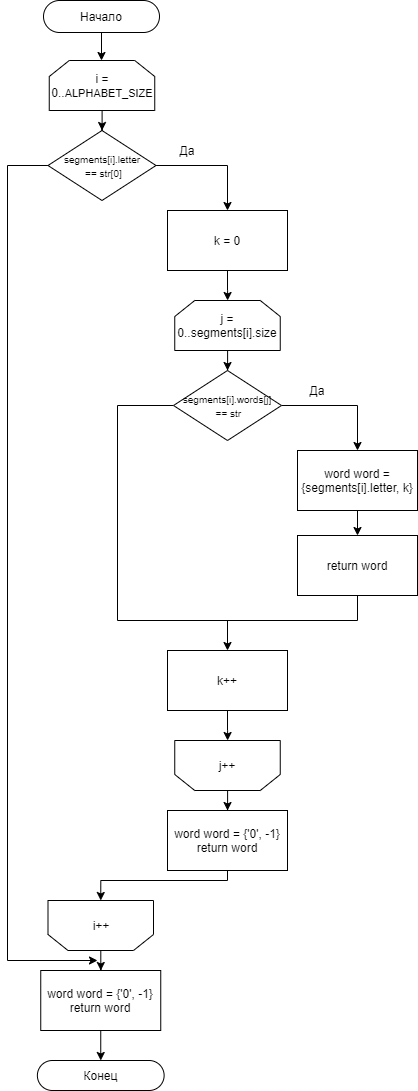
\includegraphics[scale=0.6]{source/segments.png}}
		\caption{Схема алгоритма поиска по сегментам}
	\end{figure}
	\clearpage
	
	\subsection*{Вывод}
	\addcontentsline{toc}{subsection}{Вывод}
	В данном разделе были рассмотрены схемы алгоритмов.
	\newpage
	
	\section{Технологический раздел}
	В данном разделе даны общие требования к программе, средства реализации и сама реализация алгоритмов.
	
	\subsection{Общие требования}
	Требования к вводу:
	\begin{enumerate}
		\item[1)] вводится слово;
		\item[2)] в первых 2 алгоритмах результатом будет являться ключ (в первом по обычному словарю, а во втором по отсортированному словарю), в третьем результатом будет являться ключ (первая буква или же сегмент) и индекс слова в сегменте. 
	\end{enumerate}\par
	Требования к программе
	\begin{enumerate}
		\item[1)] при вводе слова, которого нет в словаре, программа не должна завершиться аварийно;
		\item[2)] ключ или же ключ-индекс должны быть корректными (соответствовать нужному слову).
	\end{enumerate}\par

	\subsection{Средства реализации}
	В лабораторной работе был использован язык $C$++\hyperref[CPlusPlus]{[1]}, так как он известен, и на нём было написано множество предыдущих работ.
	
	Среда разработки - $Qt$\hyperref[Cute]{[2]}.
	
	Для замеров процессорного времени была использована функция $clock()$\hyperref[CLOCK]{[3]}.
	\newpage
	
	\subsection{Листинг кода программы}
	В Листинге 1 реализован алгоритм полного перебора слов.
	
	\begin{lstlisting}[caption=Алгоритм полного перебора слов]
		int Dictionary::brute_force(std::string str)
		{
			for (size_t i = 0; i < size; i++)
			{
				if (str == content[i])
				return i;
			}
			
			return -1;
		}	
	\end{lstlisting}
	
	В Листинге 2 реализован алгоритм двоичного поиска
	
	\begin{lstlisting}[caption=Алгоритм двоичного поиска]
		int Dictionary::binary_find(std::string str)
		{
			int left = 0;
			int right = size;
			int mid = 0;
			
			while(left <= right)
			{
				mid = (left + right) / 2;
				
				if (str < content[mid])
				right = mid - 1;
				else if (str > content[mid])
				left = mid + 1;
				else return  mid;
			}
			return -1;
		}		
	\end{lstlisting}
	
	В Листинге 3 реализован алгоритм поиска по сегментам
	
	\begin{lstlisting}[caption=Алгоритм поиска по сегментам]
		SegDictionary::SegDictionary(Dictionary& dic)
		{
			char alphabet[] = {'e', 't', 'a', 'o', 'i', 'n', 's', 'h', 'r', 'd', 'l', 'c',\
				'u', 'm', 'w', 'f', 'g', 'y', 'p', 'b', 'v', 'k', 'x', 'j', \
				'q', 'z'};
			
			for (size_t i = 0; i < ALPHABET_SIZE; i++)
			{
				char cur_letter = alphabet[i];
				size_t amount = 0;
				segment seg;
				seg.letter = cur_letter;
				
				for (size_t j = 0; j < dic.size; j++)
				{
					if (dic.content[j][0] == cur_letter)
					{
						seg.words[amount] = dic.content[j];
						amount++;
					}
				}
				
				seg.size = amount;
				segments[i] = seg;
			}
		}
	\end{lstlisting}

	\subsection*{Вывод}
	\addcontentsline{toc}{subsection}{Вывод}
	В данном разделе были даны общие требования к программе, описаны средства реализации, а также реализованы алгоритмы поиска по словарю.
	
	
	\section{Экспериментальный раздел}
	В данном разделе представлены результаты работы программы и приведен анализ времени работы алгоритмов.
	
	\subsection{Примеры работы программы}
	На Рисунке 4 представлен пример работы программы.
	\begin{figure}[h!]
		\centering{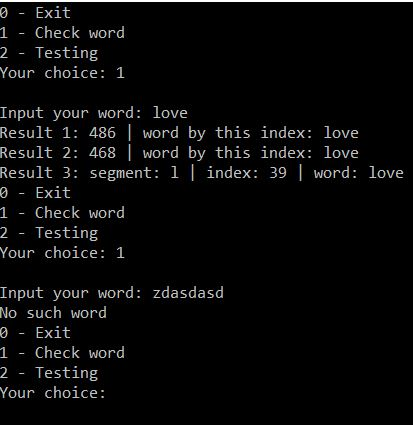
\includegraphics[scale=1]{source/example.jpg}}
		\caption{Примеры работы программы}
	\end{figure}
	
	\subsection{Описание экспериментов}
	Производится замер времени для $n + 1$ возможных случаев, где $n$ - длина словаря.\par
	На Рисунке 5 представлены результаты сравнения трех алгоритмов поиска.
	\begin{figure}[h!]
		\centering
		\begin{tikzpicture}[object/.style={thin,double,<->}]
			
			\begin{axis}[
				axis lines = left,
				xlabel = $\textit{индекс слова в словаре}$,
				ylabel = {$\textit{кол-во тиков}$},
				legend pos=north west,
				ymajorgrids=true
				]
				\addplot[color=red] table[x index=0, y index=1] {source/brute_force.dat}; 
				\addplot[color=orange] table[x index=0, y index=1] {source/binary_find.dat};
				\addplot[color=blue, mark=square] table[x index=0, y index=1] {source/find_in_segment.dat};
				
				\addlegendentry{Полный перебор}
				\addlegendentry{Бинарный поиск}
				\addlegendentry{Поиск по сегментам}				
			\end{axis}
		\end{tikzpicture}
		
		\caption{Результаты замеров процессорного времени.}
		\label{Test1}
	\end{figure}\par

	\subsection*{Вывод}
	\addcontentsline{toc}{subsection}{Вывод}
	По результатам тестирования выяснилось, что бинарный поиск наиболее стабилен по времени, но поиск по сегментам в некоторых случаях работает быстрее. По графику алгоритма поиска по сегментам можно увидеть резкие скачки. Это происходит из-за того, что слово в находится в конце сегмента. Самым медленным оказался полный перебор, у которого время работы пропорционально индексу слова в словаре. 
	
	\clearpage
	\section{Заключение}
	\addcontentsline{toc}{section}{Заключение}	
	В ходе выполнения данной лабораторной работы были изучены три алгоритмы поиска по словарю. Были описаны все алгоритмы и реализованы. Также были изучены способы хранения слов, то есть в случаях первого и второго алгоритмов слова хранились в массивах, а в третьем хранилось по сегментам. Сравнили время работы алгоритмов, в результате которого стало понятно, что наиболее стабильным по времени оказался бинарный поиск, но в некоторых случаях поиск по сегментам может быть быстрее.
	\clearpage

	\newpage	
	\section*{Литература}
	\addcontentsline{toc}{section}{Литература}
		
	\begin{enumerate}
		\label{CPlusPlus}
		\item[1)] Бьерн Страуструп. Язык программирования С++. -URL:\par 
		\href{https://codernet.ru/books/c_plus/bern_straustrup_yazyk_programmirovaniya_c_specialnoe_izdanie/}
		{https://codernet.ru/books/c\_plus/bern\_straustrup\_yazyk\_programmirovaniya\_
			c\_specialnoe\_izdanie/}\par(дата обращения:
		01.10.2020). Текст: электронный.
		
		\label{Cute}
		\item[2)] Qt. -URL:\par
		\href{https://www.qt.io/}{https://www.qt.io/} (дата обращения: 01.10.2020). Текст: электронный.
		
		\label{CLOCK}
		\item[3)] Функция $clock$. -URL:\par
		\href{https://docs.microsoft.com/ru-ru/cpp/c-runtime-library/reference/clock?view=vs-2019}{https://docs.microsoft.com/ru-ru/cpp/c-runtime-library/reference/clock?view=vs-2019} (дата обращения:
		01.10.2020). Текст: электронный.
		
		\item[4)] Полный перебор. -URL:\par
		\href{https://spravochnick.ru/informatika/algoritmizaciya/algoritm_polnogo_perebora/}{https://spravochnick.ru/informatika/algoritmizaciya/algoritm\_polnogo\_perebora/} (дата обращения:
		28.12.2020). Текст: электронный.
		
		\item[5)] Бинарный поиск. -URL:\par
		\href{https://prog-cpp.ru/search-binary/}{https://prog-cpp.ru/search-binary/} (дата обращения: 28.12.2020). Текст: электронный.
		
		\item[6)] Словарь. -URL:\par
		\href{http://gramota.ru/slovari/types/17_2}{http://gramota.ru/slovari/types/17\_2} (дата обращения: 28.12.2020). Текст: электронный.	
		
	\end{enumerate}
	\label{Litre}	
	
\end{document}